\begin{frame}{Mass of \chiboneTwoP in $\chib \to \TwoS \gamma$ decay}
\begin{center}
\setlength{\unitlength}{1mm}
\begin{picture}(70,50)
  %
\put(0,0){
  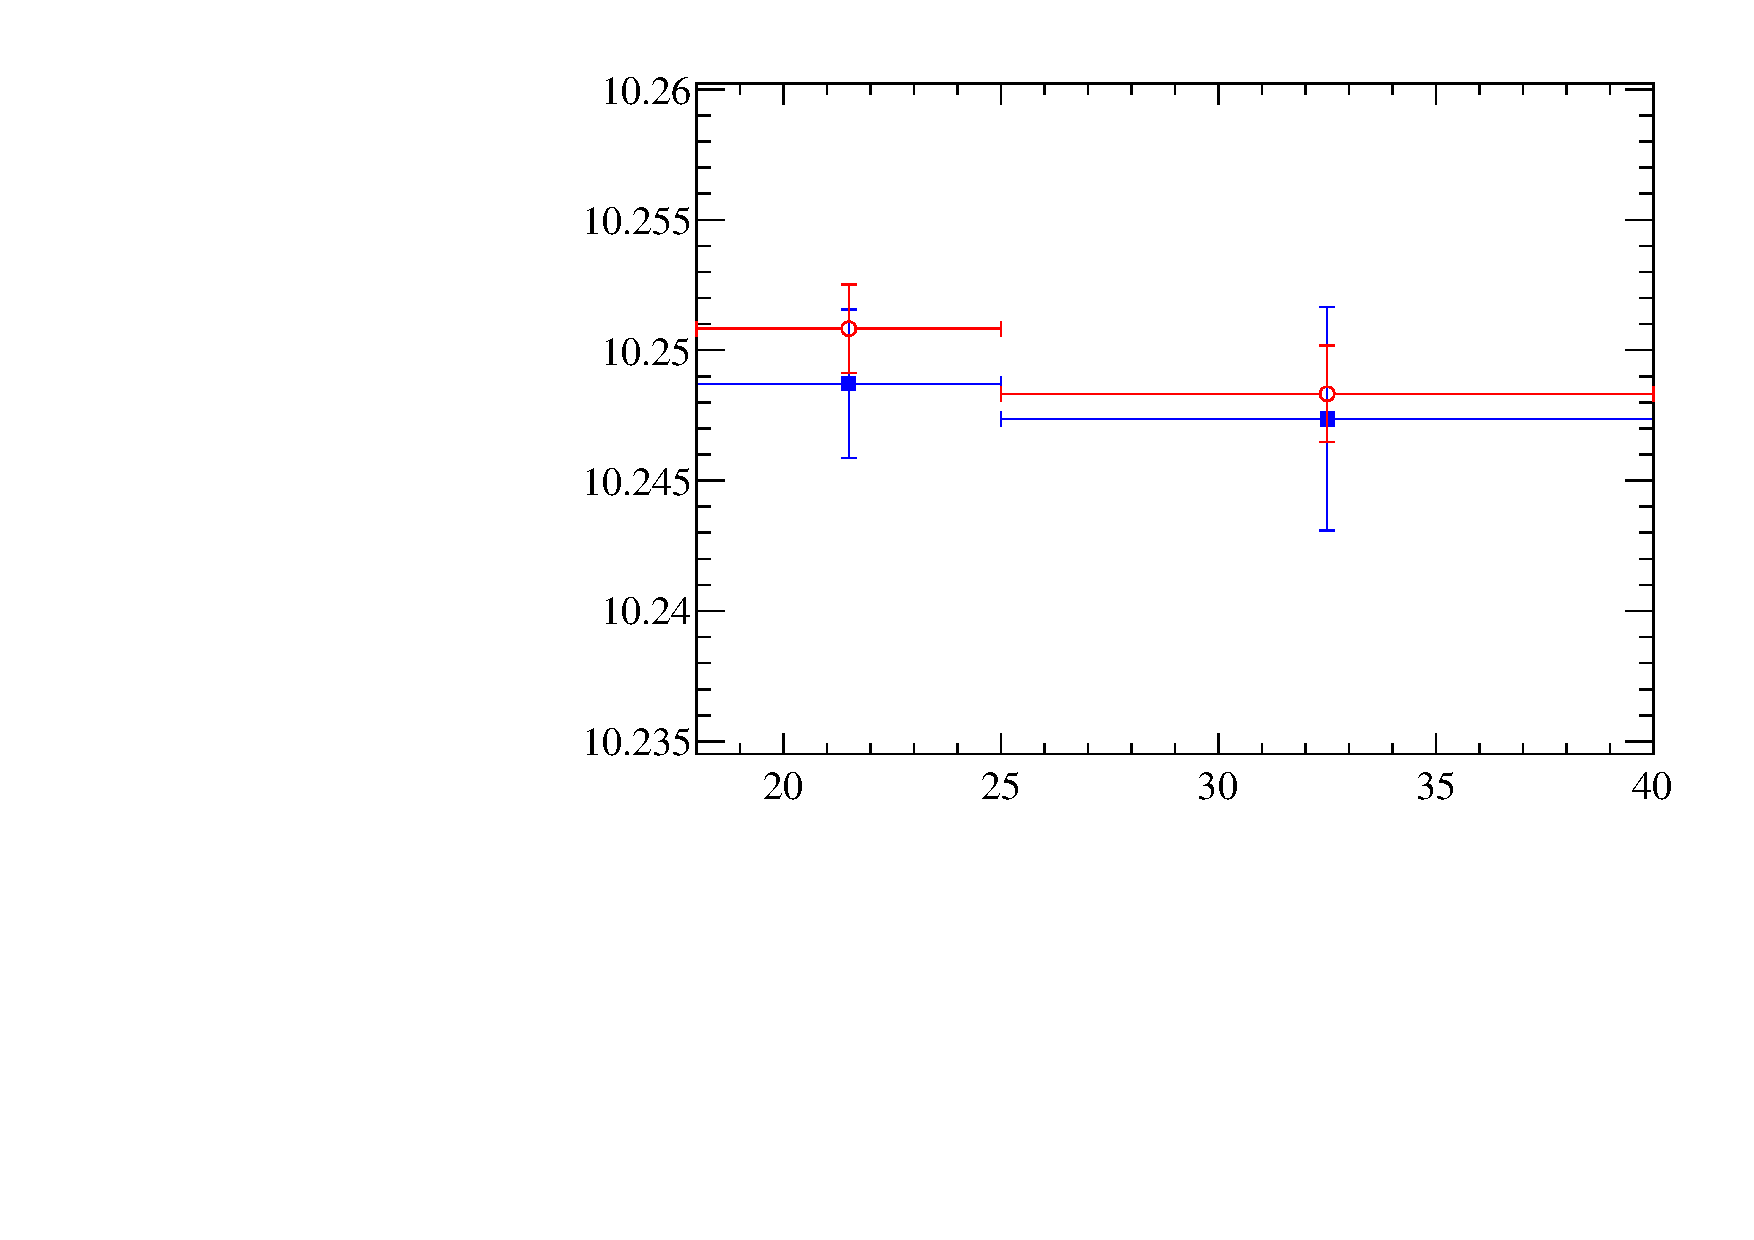
\includegraphics[width=70mm, height=50mm]{chib2s-m/m2p_2s}
}

\put(27, 40){\textcolor{blue}{\sqs=7\tev}, \textcolor{red}{\sqs=8\tev}}
\put(0,12){\begin{sideways}\chiboneTwoP mass \gevcc\end{sideways}}
\put(20,1){$p_T(\Upsilon) \left[\gevc\right]$}

%\put(0,12){\begin{sideways}Candidates\end{sideways}}
%\put(17,0){$p_T(\Upsilon) \left[\gevc\right]$}
%\put(35,30){\ThreeS}

%    \put(12,0){\tiny $m(\mumu) \left[\gevcc\right]$}
     
%\graphpaper[5](0,0)(50, 40)        
\end{picture}


In this study the mass of \chiboneTwoP was fixed to \textcolor{blue}{10249} \mevcc.

\end{center}
\end{frame}
